\documentclass[11pt,a4paper,oneside]{book}

% Pacotes essenciais para padrão acadêmico internacional
\usepackage[utf8]{inputenc}
\usepackage[T1]{fontenc}
\usepackage{lmodern}
\usepackage{amsmath,amssymb,amsfonts}
\usepackage{graphicx}
\usepackage{booktabs}
\usepackage{microtype}
\usepackage{algorithm}
\usepackage{algpseudocode}
\usepackage{tabularx}
\usepackage{adjustbox}
\usepackage{pdflscape}
\usepackage{array}
\usepackage{longtable}
\usepackage{geometry}
\usepackage{xcolor}
\usepackage{hyperref}
\usepackage{fancyhdr}
\usepackage{titlesec}
\usepackage{cite}
\setlength{\emergencystretch}{3em}
\raggedbottom

% Configuração de margens e geometria
\geometry{
    a4paper,
    top=28mm,
    bottom=28mm,
    left=30mm,
    right=25mm
}

% Cores acadêmicas
\definecolor{primaryblue}{RGB}{2, 132, 199}
\definecolor{darknavy}{RGB}{8, 19, 36}
\definecolor{academicgray}{RGB}{100, 116, 139}

\hypersetup{
    colorlinks=true,
    linkcolor=primaryblue,
    citecolor=primaryblue,
    urlcolor=primaryblue,
    pdftitle={Evidence-Based Environmental CVSS v4.0 Prioritization: An Explainable AI Watcher Architecture with Human-in-the-Loop Governance},
    pdfauthor={Wagner Santos, HelpUS Security Research}
}

% Cabeçalhos e rodapés
\pagestyle{fancy}
\fancyhf{}
\fancyhead[L]{\small\color{academicgray}\ifnum\value{chapter}>0 \chaptername~\thechapter\fi}
\fancyhead[R]{\small\color{academicgray}HelpUS Research Monograph}
\setlength{\headheight}{14pt}
\fancyfoot[C]{\thepage}
\renewcommand{\headrulewidth}{0.4pt}

% Auto-generated by scripts/reproduce_historical_fisher.py; do not edit manually.
\newcommand{\HistFisherPScientific}{4.2235 \times 10^{-6}}
\newcommand{\HistSampleOR}{3.388}
\newcommand{\HistConditionalOR}{3.377}
\newcommand{\HistConditionalCILow}{1.913}
\newcommand{\HistConditionalCIHigh}{6.184}


\begin{document}

% Capa Acadêmica
\begin{titlepage}
    \centering
    \vspace*{2cm}
    
    {\Huge\bfseries\color{darknavy} Evidence-Based Environmental CVSS v4.0 Prioritization\par}
    \vspace{0.8cm}
    {\Large\itshape An Explainable AI Watcher Architecture with Grounded Telemetry and Human-in-the-Loop Governance\par}
    
    \vspace{2.5cm}
    {\large\bfseries Wagner Santos\par}
    \vspace{0.2cm}
    {\normalsize SecOps Research Lead, HelpUS Security Group\par}
    {\normalsize \texttt{wagner@helpusbr.com}\par}
    
    \vfill
    {\large\bfseries Comprehensive Technical Reference Monograph \& Companion Book\par}
    \vspace{0.4cm}
    {\small Prepared for IEEE International Conference on AI in Cybersecurity (ICAIC 2027) Submissions\par}
    \vspace{0.8cm}
    {\normalsize October 2026\par}
\end{titlepage}

\frontmatter

\tableofcontents
\listoffigures
\listoftables

\chapter{Executive Summary}
This research monograph provides a comprehensive mathematical, architectural, and empirical reference for automated vulnerability prioritization under the FIRST Common Vulnerability Scoring System (CVSS) v4.0 specification. 

Addressing the operational limitations of using source CVSS assessments without organization-specific context, we introduce the HelpUS Framework: a system integrating network-topology evidence, an explainable evidence-constrained deterministic inference pipeline, specification-conformant CVSS v4.0 scoring, and a Human-in-the-Loop (HITL) review gate. The governance workflow is designed to support auditability and human oversight; it does not by itself establish compliance with NIST, ISO, PCI-DSS, or other frameworks. 

The current 30-scenario Dataset B is a development benchmark used for architectural verification and regression testing; it is not confirmatory evidence of external generalization. A pinned FIRST calculator reference corpus has been fully verified across all 486,472 test cases against official FIRST commit d766d0c8ab4368b67bf27dd0e411eb481f05fdbb with zero mismatches, successfully closing the calculator conformance gate (G1). Dataset B source provenance has been migrated to a schema that separates provider-reported Base values from scores recomputed from full source vectors, and all manuscript tables must be regenerated from that canonical source before freeze. Engine-level timing measurements are reported separately from historical human-session timings and are not treated as a like-for-like end-to-end speedup. Confirmatory claims remain pending independent held-out evaluation (Datasets C1/C2), expert adjudication, and applicable ethics determination. Web-layer audit-receipt canonicalization and authorization controls remain separate engineering claims that require their own conformance and security evidence.

\mainmatter

\chapter{Introduction: The Vulnerability Prioritization Crisis}
\label{chap:introduction}

\section{The Threat Landscape and Alert Fatigue}
In contemporary enterprise architectures, vulnerability management programs are confronted with an unprecedented volume of Common Vulnerabilities and Exposures (CVEs). Organizations routinely receive tens of thousands of automated scanner findings per month. In practice, operational security teams (SecOps) cannot patch all reported defects within typical service level agreements (SLAs).

The primary challenge lies in \textbf{alert inflation}: conventional scanners evaluate vulnerability severity based heavily on source CVSS assessments published by vulnerability authorities and commonly indexed by services such as the National Vulnerability Database (NVD)~\cite{first_cvss_v4}. A remote code execution (RCE) defect assigned a CVSS Base score of 9.8 is treated as an existential emergency regardless of whether the affected host is an edge-facing payment gateway or an isolated development sandbox accessible only over a local loopback interface.

\begin{figure}[htbp]
    \centering
    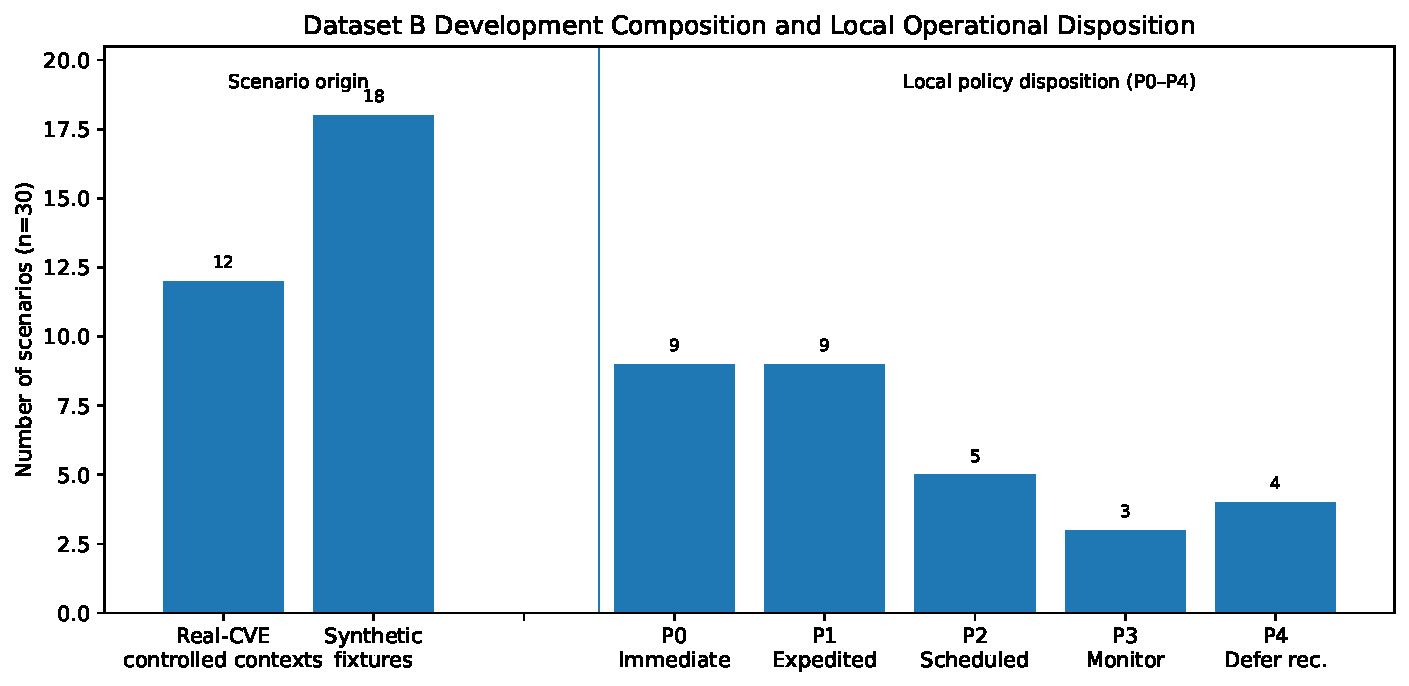
\includegraphics[width=0.96\linewidth]{figures/fig1_dataset_composition.pdf}
    \caption{Dataset B development composition shown without conflating CVSS severity with local policy. The left group identifies scenario origin (12 real-CVE records embedded in controlled contexts and 18 synthetic fixtures); the right group shows legacy local P0--P4 development-policy dispositions. The chart is descriptive development evidence only; it is not an accuracy, false-positive, or held-out validation result.}
    \label{fig:severity_redistribution}
\end{figure}

\section{The Dilemma of Intrinsic Severity vs. Operational Context}
The fundamental mathematical and semantic boundary of vulnerability management is delineated by two concepts:
\begin{enumerate}
    \item \textbf{Base Severity ($S_{\text{base}}$):} Represents vulnerability characteristics that are intended to remain independent of a specific organization's environment. Local compensating controls and business requirements are deliberately outside the Base metric group.
    \item \textbf{Contextual Environmental Severity ($S_{\text{env}}$):} Represents a CVSS Environmental result after organization-specific modified metrics and security requirements have been documented. It is a contextual severity score, not a complete probabilistic risk estimate.
\end{enumerate}

FIRST CVSS v4.0 defines Environmental metrics so that local conditions can be represented explicitly. Applying those metrics at scale may require analysts to reconcile vulnerability records with topology, reachability, asset requirements, and compensating controls. Prior empirical work shows that such contextual assessment becomes error-prone in complex network scenarios~\cite{santos2017estimating}. This work therefore studies whether verified operational evidence can support a more reproducible and auditable recommendation process.

\section{The HelpUS Solution and Research Objectives}
This work introduces the \textbf{HelpUS CVSS Framework}, an evidence-grounded decision architecture that derives \emph{candidate} CVSS v4.0 Environmental metrics from verified operational evidence and then delegates numerical scoring to a specification-conformant CVSS v4.0 calculator. 

Our core contributions are structured as follows:
\begin{itemize}
    \item \textbf{Tripartite Evidence Contract:} Preservation of the source CVSS assessment vector and nomenclature alongside the contextual result and its provenance, supporting auditability without overwriting the original assessment.
    \item \textbf{Deterministic AI Watcher:} An evidence-constrained inference layer that recommends candidate Environmental metrics and abstains when the evidence is incomplete or contradictory.
    \item \textbf{Inverse Environmental Optimization (What-If Solver):} A constrained combinatorial solver that deduces the minimal set of compensating controls required to meet organizational risk thresholds.
    \item \textbf{Policy-as-Code Virtual Patching:} Synthesis of candidate Linux \texttt{iptables}, cloud security-group, and WAF controls that require validation and Human-in-the-Loop approval before production deployment.
    \item \textbf{Reachability-Adjusted EPSS Heuristic:} A clearly labeled heuristic for combining global exploit-likelihood information with local reachability evidence; it is not presented as a calibrated posterior probability.
    \item \textbf{Human-in-the-Loop (HITL) Governance \& SLA Clock:} An auditable 4-step review workflow designed to support organizational governance and alignment with relevant NIST/ISO practices, with tamper-evident provenance and configurable SLA policy.
    \item \textbf{Empirical Scientific Benchmark:} A 30-scenario preliminary benchmark reporting priority redistribution, traceability, abstention behavior, and engine-level latency; accuracy claims require an independently adjudicated expert reference set.
\end{itemize}

\chapter{FIRST CVSS v4.0 Specification and Theoretical Foundations}
\label{chap:cvss_foundations}

\section{Evolution of Vulnerability Metrics: CVSS v2 to v4.0}
The Common Vulnerability Scoring System (CVSS), maintained by the Forum of Incident Response and Security Teams (FIRST), represents the global standard for vulnerability characterization~\cite{first_cvss_v4}. While CVSS v2 and v3.1 provided foundational metrics, they suffered from significant metric compression and inadequate separation between threat intelligence and environmental mitigations.

In CVSS v4.0, FIRST established a strict taxonomy comprising four distinct nomenclature groups:
\begin{itemize}
    \item \textbf{CVSS-B (Base):} Measures intrinsic qualities that are constant over time and across user environments.
    \item \textbf{CVSS-BT (Base + Threat):} Factors in temporal exploit maturity (Attacked, Proof-of-Concept, Unreported).
    \item \textbf{CVSS-BE (Base + Environmental):} Factors in local system characteristics, compensating mitigations, and organizational requirements.
    \item \textbf{CVSS-BTE (Base + Threat + Environmental):} The comprehensive score incorporating all metric groups.
\end{itemize}

\section{Environmental Vector Decomposition}
The environmental metric group modifies Base metrics according to the defensive reality of the target asset. The formal environmental metric vector comprises two primary subsets:

\subsection{Modified Base Metrics}
Defenders alter the base vector when local architectural controls change the attack surface:
\begin{equation}
    \text{Vector}_{\text{modified}} = \{\text{MAV}, \text{MAC}, \text{MAT}, \text{MPR}, \text{MUI}, \text{MVC}, \text{MVI}, \text{MVA}, \text{MSC}, \text{MSI}, \text{MSA}\}
\end{equation}

Among these, the \textbf{Modified Attack Vector (MAV)} represents the most impactful lever in segmented infrastructure:
\begin{itemize}
    \item $\text{MAV:Network (N)} \rightarrow$ Exploitation can be performed remotely through a network protocol stack; the attacker may be one or more network hops away. Internet exposure is one possible case, but is not required.
    \item $\text{MAV:Adjacent (A)} \rightarrow$ Exploitation requires access to a logically or physically adjacent network context, such as the same constrained broadcast or proximity domain.
    \item $\text{MAV:Local (L)} \rightarrow$ Exploitation requires local access to the vulnerable system or a local execution context; this is distinct from physical manipulation.
    \item $\text{MAV:Physical (P)} \rightarrow$ Exploitation requires physical interaction with the vulnerable component. The authoritative FIRST specification remains the normative definition~\cite{first_cvss_v4}.
\end{itemize}

\subsection{Security Requirements (CR, IR, AR)}
Security Requirements customize the impact based on the asset's business criticality and regulatory classification:
\begin{align}
    \text{CR} &\in \{\text{High}, \text{Medium}, \text{Low}, \text{Not Defined}\} \\
    \text{IR} &\in \{\text{High}, \text{Medium}, \text{Low}, \text{Not Defined}\} \\
    \text{AR} &\in \{\text{High}, \text{Medium}, \text{Low}, \text{Not Defined}\}
\end{align}

Security Requirements are organization-specific. Regulatory or business scope (including PCI-DSS) may inform a documented organizational mapping policy, but the external standard does not by itself mandate particular CVSS values such as $\text{CR:High}$ or $\text{IR:High}$. Any such mapping in HelpUS must therefore be explicit, reviewable, and attributable to local policy.

\section{The Mathematical Formula and Macro-Vectors}
Unlike CVSS v3.1, CVSS v4.0 uses a MacroVector lookup-and-interpolation architecture~\cite{first_cvss_v4}. The equivalence groups defined by FIRST are not a simple one-to-one partition of the named Base, Threat, and Environmental metric groups. The normative grouping is:
\begin{itemize}
    \item $EQ_1$: AV / PR / UI.
    \item $EQ_2$: AC / AT.
    \item $EQ_3$: VC / VI / VA.
    \item $EQ_4$: SC / SI / SA.
    \item $EQ_5$: E (Exploit Maturity).
    \item $EQ_6$: the vulnerable-system impact metrics VC / VI / VA evaluated together with the Environmental Security Requirements CR / IR / AR.
\end{itemize}
FIRST further specifies that $EQ_3$ and $EQ_6$ are not independent and are considered jointly during MacroVector scoring. Modified Environmental metrics influence the effective metric values used by the scoring process; they should not be described as a separate serialized ``EQ6 modified-impact'' group. The FIRST specification remains the normative source for the boolean level definitions and interpolation algorithm~\cite{first_cvss_v4}.

The calculated environmental score $S_{\text{env}}$ is bounded by:
\begin{equation}
    0.0 \le S_{\text{env}} \le 10.0
\end{equation}
The score variation $\Delta$ between the source score $S_{\text{source}}$ and the contextual environmental score is defined as:
\begin{equation}
    \Delta = S_{\text{env}} - S_{\text{source}}
\end{equation}
A negative $\Delta$ indicates that the contextual CVSS result is numerically lower than the source score, whereas a positive $\Delta$ indicates a higher contextual result. Neither direction, by itself, establishes operational risk acceptance, regulatory status, or correctness.

\section{Historical Evidence on Human Difficulty in Environmental Scoring}
\label{sec:human_failure_baseline}
Environmental scoring requires assessors to combine vulnerability semantics with organization-specific system and network context. Allodi et al.~\cite{santos2017estimating} studied this assessment difficulty in a controlled 2017 experiment involving $n=29$ MSc students and enterprise network layouts derived from PCI-DSS compliance literature~\cite{williams2014pci}. The study predates CVSS v4.0 and therefore serves here as a historical human-factors baseline rather than a v4.0 ground truth.


The empirical findings reported by Allodi et al.~\cite{santos2017estimating} provide three observations that motivate the HelpUS architecture:
\begin{enumerate}
    \item \textbf{Network Complexity Destroys Human Accuracy ($H2_0$ Rejected):}
    In a simple, flat network layout, human participants achieved an acceptable correctness rate of $83\%$ ($96/116$ correct scores). However, once network segmentation was introduced to satisfy PCI-DSS scoping requirements (VLANs, DMZs, and access control lists), the human correctness rate collapsed to $59\%$ ($136/232$ correct). Fisher's exact test confirmed the overwhelming statistical significance of this degradation:
    \begin{equation}
        p = 4.2 \times 10^{-6}, \quad \text{Odds Ratio} = 3.4, \quad 95\% \text{ CI} = [1.91, 6.18]
    \end{equation}
    Human analysts are over three times more likely to miscalculate environmental scores in a modern segmented architecture than in an obsolete flat network.

    \item \textbf{System and Infrastructure Vulnerabilities Induce Severe Error ($H1_0$ Rejected):}
    The experiment revealed a profound disparity between application-level vulnerabilities (APP) and system/infrastructure-level vulnerabilities (SYS). In segmented networks, application vulnerabilities (e.g., browser or office suites) maintained a $72.4\%$ correctness rate, whereas system-level vulnerabilities (e.g., Windows RDP and Cisco core switches) suffered a disastrous error rate of $55.2\%$ ($p = 3.2 \times 10^{-5}$, Odds Ratio $= 3.2$).
    
    Most critically, for core network switches implementing Access Control Lists on top of VLANs (specifically Cisco IOS defects CVE-2016-6441 and CVE-2016-6428), \textbf{between 86\% and 90\% of human assessors made critical scoring errors}. Human analysts consistently failed to comprehend whether a vulnerable routing appliance acts as an attack target or as a protective boundary for systems behind it.

    \item \textbf{Synthetic Score-Space Sensitivity:}
    A Monte Carlo simulation of $10,000$ sampled Environmental metric combinations illustrates that different contextual assumptions can produce a broad score space. This simulation is a sensitivity illustration only; it does not measure human fatigue or reproduce the empirical participant distribution in Allodi et al. The simulation is therefore treated as a separate sensitivity exercise rather than evidence about participant behavior.
\end{enumerate}

Allodi et al.~\cite{santos2017estimating} concluded with an explicit challenge to the research community: because network topologies cannot be simplified without sacrificing security, \textbf{environmental vulnerability assessment cannot scale without automated data integration and automated topological reasoning engines}. 

The HelpUS AI Watcher framework was engineered specifically to solve the challenge formulated by Allodi et al., replacing manual guesswork with deterministic symbolic reasoning .


\chapter{Architecture of the HelpUS AI Watcher Engine}
\label{chap:architecture}

\section{System Architecture Overview}
The HelpUS framework operates as an automated bridge between network telemetry and vulnerability prioritization. Its design goal is to constrain metric recommendations to explicit evidence and deterministic rules. Generative components, when used for explanation or interface assistance, are not permitted to alter the CVSS vector without the same evidence checks and review policy. The earlier radar-style ``maturity benchmark'' has been removed because heterogeneous dimensions such as traceability, speed, and governance do not share a defensible common percentage scale.

\section{The Tripartite Evidence Contract}
A foundational principle of the HelpUS engine is that the source CVSS assessment (including its vector, nomenclature, provider, and reported score semantics) must never be overwritten, hidden, or artificially compressed. Instead, every assessment produces a \textbf{Tripartite Evidence Contract} represented formally by the tuple:
\begin{equation}
    \mathcal{C} = \langle \mathcal{O}_{\text{source}}, \mathcal{E}_{\text{context}}, \mathcal{V}_{\text{evidence}} \rangle
\end{equation}
where:
\begin{itemize}
    \item $\mathcal{O}_{\text{source}} = \{S_{\text{source}}, \text{Severity}_{\text{source}}, \mathbf{v}_{\text{source}}, \text{Provider}, \text{Nomenclature}\}$ preserves the source assessment and provenance without implying that NVD, a CNA, or FIRST authored every displayed score.
    \item $\mathcal{E}_{\text{context}} = \{S_{\text{env}}, \text{Severity}_{\text{env}}, \mathbf{v}_{\text{env}}, \Delta_{\text{score}}, \Delta_{\text{sev}}, \text{Provenance}, \mathcal{K}_{\text{citations}}\}$ specifies the derived contextual CVSS result; operational disposition is produced separately by a versioned organizational policy.
    \item $\mathcal{V}_{\text{evidence}} = \{I_{\text{route}}, N_{\text{vlan}}, F_{\text{acl}}, P_{\text{compliance}}, C_{\text{compensating}}, B_{\text{criticality}}\}$ documents the verified state of operational controls.
\end{itemize}

\section{Two-Stage Deterministic Prioritization Pipeline}
\label{sec:two_stage_pipeline}
Contrary to naive heuristics that apply arbitrary static deltas to base scores, the HelpUS engine strictly decouples \textbf{symbolic metric inference} from \textbf{standard score computation}. The architecture functions as a two-stage deterministic pipeline:
\begin{enumerate}
    \item \textbf{Stage 1: Evidence-Grounded Metric Deduction:} The engine maps physical and logical network telemetry into candidate CVSS v4.0 environmental metrics ($\text{MAV}, \text{MAC}, \text{MPR}, \text{CR}, \text{IR}, \text{AR}$).
    \item \textbf{Stage 2: Specification-Conformant CVSS v4.0 Scoring:} Candidate Environmental metrics are combined with the preserved source vector to construct a valid CVSS v4.0 vector. Numerical scoring is delegated to a pinned calculator implementation whose behavior must be validated against FIRST reference resources before confirmatory evaluation~\cite{first_cvss_v4}.
\end{enumerate}

Algorithm~\ref{alg:metric_inference} formalizes this two-stage process. The observed delta $\Delta_{\text{score}} = S_{\text{env}} - S_{\text{source}}$ is strictly an emergent mathematical consequence of the FIRST specification, never an ad-hoc arithmetic rule.

\begin{algorithm}[H]
\caption{Evidence-Grounded CVSS v4.0 Environmental Metric Inference}
\label{alg:metric_inference}
\begin{algorithmic}[1]
\footnotesize
\Require Source CVSS vector $\mathbf{v}_{\text{source}}$, versioned evidence $\mathcal{V}_{\text{evidence}}$, topology graph $\mathcal{G}$, organizational policy $\Pi$
\Ensure Either \texttt{HUMAN\_REVIEW\_REQUIRED}, or canonical contextual vector $\mathbf{v}_{\text{env}}$ and score $S_{\text{env}}$
\State $\mathcal{K} \gets \emptyset$
\If{$\text{Missing}(\mathcal{V}_{\text{evidence}}) \lor \text{Stale}(\mathcal{V}_{\text{evidence}}) \lor \text{Insufficient}(\mathcal{V}_{\text{evidence}}) \lor \text{Conflicting}(\mathcal{V}_{\text{evidence}})$}
    \State \Return \texttt{HUMAN\_REVIEW\_REQUIRED}
\EndIf
\State $\mathbf{v}_{\text{cand}} \gets \text{ExtractCandidateEnvironmentalMetrics}(\mathbf{v}_{\text{source}})$
\Comment{Topology-aware candidate MAV}
\If{$\text{RequiresPhysicalInteraction}(h, \mathcal{V}_{\text{evidence}})$}
    \State $\mathbf{v}_{\text{cand}}.\text{MAV} \gets \text{Physical}$
    \State $\mathcal{K} \gets \mathcal{K} \cup \{\text{``MAV:P - physical interaction required''}\}$
\ElsIf{$\text{IsLoopbackOrLocalOnly}(h, \mathcal{V}_{\text{evidence}})$}
    \State $\mathbf{v}_{\text{cand}}.\text{MAV} \gets \text{Local}$
    \State $\mathcal{K} \gets \mathcal{K} \cup \{\text{``MAV:L - local execution/access required''}\}$
\ElsIf{$\text{IsAdjacentOnlyDomain}(h, \mathcal{G})$}
    \State $\mathbf{v}_{\text{cand}}.\text{MAV} \gets \text{Adjacent}$
    \State $\mathcal{K} \gets \mathcal{K} \cup \{\text{``MAV:A - verified adjacent-only domain''}\}$
\ElsIf{$\text{HasVerifiedRoutedPath}(h, \mathcal{G})$}
    \State $\mathbf{v}_{\text{cand}}.\text{MAV} \gets \text{Network}$
    \State $\mathcal{K} \gets \mathcal{K} \cup \{\text{``MAV:N - verified routed reachability''}\}$
\Else
    \State \Return \texttt{HUMAN\_REVIEW\_REQUIRED}
\EndIf
\If{$\text{HasFirewallOrWafEvidence}(h, \mathcal{V}_{\text{evidence}})$}
    \State $\mathcal{K} \gets \mathcal{K} \cup \{\text{``firewall/WAF recorded; MAC unchanged by presence alone''}\}$
\EndIf
\If{$\text{ExploitPreconditionsSupportHighComplexity}(\mathcal{V}_{\text{evidence}})$}
    \State $\mathbf{v}_{\text{cand}}.\text{MAC} \gets \text{High}$
\EndIf
\Comment{Organization-specific requirements}
\If{$\text{HasApprovedRequirementMapping}(\Pi, \mathcal{V}_{\text{evidence}})$}
    \State $(\text{CR},\text{IR},\text{AR}) \gets \text{ApplyVersionedPolicy}(\Pi, \mathcal{V}_{\text{evidence}})$
    \State $\mathcal{K} \gets \mathcal{K} \cup \{\text{``versioned organizational requirement policy''}\}$
\EndIf
\State $\mathbf{v}_{\text{env}} \gets \text{SynthesizeCanonicalVector}(\mathbf{v}_{\text{source}}, \mathbf{v}_{\text{cand}})$
\State $S_{\text{env}} \gets \text{ComputeCVSS40Pinned}(\mathbf{v}_{\text{env}})$
\State $S_{\text{source}} \gets \text{ComputeOrPreserveSourceScore}(\mathbf{v}_{\text{source}})$
\State $\Delta_{\text{score}} \gets \text{round}(S_{\text{env}} - S_{\text{source}}, 1)$
\State \Return $\mathbf{v}_{\text{env}}, S_{\text{env}}, \Delta_{\text{score}}, \mathcal{K}$
\end{algorithmic}
\end{algorithm}

\section{Formal Topological Inference for Modified Attack Vector (MAV)}
\label{sec:mav_formal_table}
A critical requirement of scientific rigor is to avoid conflating the absence of direct public Internet exposure with $\text{MAV:Local}$ or $\text{MAV:Adjacent}$. An internal corporate server that lacks an external IPv4 address but is accessible across enterprise L3 routed subnets remains vulnerable via $\text{MAV:Network}$.

Table~\ref{tab:mav_inference_matrix} establishes the formal topological inference matrix implemented in the HelpUS engine.

\begin{table}[htbp]
\centering
\small
\caption{Evidence-oriented reachability conditions for candidate Modified Attack Vector (MAV) recommendations. FIRST remains the normative semantic source.}
\label{tab:mav_inference_matrix}
\begin{adjustbox}{max width=\textwidth}
\begin{tabular}{p{2.7cm}p{3.8cm}cp{4.7cm}p{2.1cm}}
\toprule
\textbf{Reachability condition} & \textbf{Observed evidence} & \textbf{Candidate} & \textbf{Rationale / limitation} & \textbf{Evidence strength} \\
\midrule
Remotely routable service & Verified routed path from an allowed remote network to the vulnerable service & $\text{MAV:N}$ & Network does not mean ``public Internet''; internal routed reachability may still satisfy Network semantics & Direct \\
Adjacent-only domain & Verified absence of L3 routing and requirement to join the same constrained L2/proximity domain & $\text{MAV:A}$ & Use only when the attack truly requires adjacency under the FIRST definition & Strong \\
Local execution context & Service/component is not remotely reachable and exploitation requires local execution/access on the vulnerable system & $\text{MAV:L}$ & Physical access is a distinct $\text{MAV:P}$ case & Direct \\
Physical interaction & Exploitation requires physical manipulation of the vulnerable component & $\text{MAV:P}$ & Must be supported by vulnerability semantics, not inferred from network isolation alone & Direct \\
Ambiguous / incomplete & Partial routes, stale telemetry, unresolved NAT/VPN/firewall state, or conflicting evidence & \textit{Abstain} & \texttt{HUMAN\_REVIEW\_REQUIRED}; preserve source priority rather than downgrade & Insufficient \\
\bottomrule
\end{tabular}
\end{adjustbox}
\end{table}

\subsection{Conservative Fail-Safe and Abstention Policy}
In security-critical operations, an erroneous vulnerability downgrade introduces material security blind spots. Therefore, the HelpUS decision engine enforces a \textbf{Conservative Fail-Safe Policy}:
\begin{align}
    &\text{Missing}(\mathcal{V}_{\text{evidence}}) \lor \text{Stale}(\mathcal{V}_{\text{evidence}}) \lor \\
    &\text{Insufficient}(\mathcal{V}_{\text{evidence}}) \lor \text{Conflicting}(\mathcal{V}_{\text{evidence}}) \nonumber\\
    &\hspace{2cm}\Longrightarrow \text{Status} \gets \texttt{HUMAN\_REVIEW\_REQUIRED}.
\end{align}
Under this policy, incomplete, stale, unknown, or contradictory evidence causes automated inference to abstain. Automatic downgrade remains disabled and a human review is required before an operational disposition is approved.

\section{Exact Combinatorial Optimization for What-If Target Remediation}
\label{sec:whatif_optimizer}
Conventional vulnerability management operates strictly in forward mode: given observed controls, it calculates the residual risk. HelpUS introduces the \textbf{What-If Target Remediation Solver}, which answers the operational engineering question: \textit{What is the exact minimal-cost set of compensating controls required to drive the environmental score below an organizational risk ceiling $\theta_{\text{target}}$?}

Formally, let $\mathbf{U} = \{c_1, c_2, \dots, c_m\}$ denote the finite universe of deployable compensating controls (e.g., VLAN microsegmentation, WAF virtual patching, egress proxy restriction, credential rotation, service isolation). Each control $c_i$ has an associated operational disruption cost $w(c_i) \in \mathbb{R}^+$. The optimization problem is formulated as:
\begin{align}
    \min_{\mathbf{c} \subseteq \mathbf{U}} \quad & \sum_{c_i \in \mathbf{c}} w(c_i) \\
    \text{subject to} \quad & S_{\text{env}}(\mathbf{c} \cup \mathcal{V}_{\text{active}}) \le \theta_{\text{target}} \nonumber
\end{align}
where $\theta_{\text{target}}$ is an organization-configured contextual-severity ceiling. Example thresholds may be used in experiments, but they are not universal risk standards.

\subsection{Exact Global Optimality via Exhaustive State Enumeration}
Unlike heuristic approximations that risk sub-optimal local minima, the HelpUS solver leverages the fact that the universe of viable architectural controls for a single workload is finite and bounded ($m \le 8$, comprising $2^m \le 256$ candidate subsets).

For the bounded candidate-control universe ($m \le 8$), the solver can enumerate at most $256$ subsets. Runtime is treated as an empirical property of the implementation and hardware and is reported only from a documented benchmark; no universal sub-millisecond timing claim is assumed here:
\begin{equation}
    \mathbf{c}^* = \arg\min_{\mathbf{c} \in \mathcal{P}(\mathbf{U})} \left\{ \sum_{c_i \in \mathbf{c}} w(c_i) \ \middle|\ S_{\text{env}}(\mathbf{c} \cup \mathcal{V}_{\text{active}}) \le \theta_{\text{target}} \right\}
\end{equation}
Within the explicitly enumerated candidate-control universe and stated cost function, exhaustive search identifies a global minimum-cost feasible subset. This does not imply global optimality over controls that were not represented in $\mathbf{U}$, and all recommended controls remain subject to validation and human approval.

\section{Policy-as-Code Virtual Patching Synthesis}
\label{sec:virtual_patching}
When software vendors require weeks to release official source-code patches, organizations face severe zero-day exposure windows. The HelpUS engine addresses this by synthesizing executable \textbf{Policy-as-Code Virtual Patches} directly from the CVSS vector decomposition.

Depending on detected network topology and service protocol, the engine synthesizes deterministic firewall and proxy candidate rules:
\begin{enumerate}
    \item \textbf{Linux Host-Level Packet Filtering (\texttt{iptables}):} Drops non-internal traffic destined to vulnerable daemon ports:
    \begin{verbatim}
    iptables -A INPUT -p tcp --dport 8080 ! -s 10.0.0.0/8 -j DROP
    \end{verbatim}
    \item \textbf{Cloud Infrastructure Security Groups (AWS CLI):} Revokes wide-open ingress rules ($0.0.0.0/0$) on public interfaces and tightens security group scopes.
    \item \textbf{Edge Application Layer Defense (Cloudflare WAF):} Synthesizes JSON filter expressions targeting exploit signatures in HTTP headers and URI payloads.
\end{enumerate}

To ensure operational stability, synthesized virtual patches are treated as \textbf{candidate compensating controls}: they undergo static syntax validation, blast-radius reachability simulation, and mandatory Human-in-the-Loop review before deployment into production.

\section{Exploratory Reachability-Adjusted EPSS Model (Future Work)}
\label{sec:contextual_epss}
The production scoring pipeline is centered on source CVSS and HelpUS-derived Environmental CVSS. A separate exploratory model considers combining EPSS with reachability evidence; it is not part of the confirmatory contribution. For historical comparison, the following notation may be used descriptively:
\begin{equation}
    \mathbf{T} = \begin{bmatrix} S_{\text{base}}^{\text{v3.1}} & S_{\text{base}}^{\text{v4.0}} & S_{\text{env}}^{\text{AI}} \end{bmatrix}^T
\end{equation}
Furthermore, while the Exploit Prediction Scoring System (EPSS)~\cite{jacobs2021exploit} provides a global probability $P(E_{\text{wild}})$ of in-the-wild exploitation, it ignores local perimeter reachability. An unauthenticated RCE on a host with zero network access has virtually zero practical exploitation probability.

A future-work prototype may compute a \textbf{Reachability-Adjusted EPSS heuristic} via:
\begin{equation}
    P(E_{\text{local}}) = P(E_{\text{wild}}) \times \Phi(\mathcal{G}_{\text{reachability}})
\end{equation}
where $\Phi(\cdot)$ is an explicitly heuristic exposure factor. Until calibrated against outcome data, the quantity must not be interpreted as a Bayesian posterior or calibrated exploitation probability and is excluded from the primary held-out evaluation.


\chapter{Dynamic Network Scanning and Topology Inference}
\label{chap:network_scanner}

\section{Real-Time Discovery Pipeline}
Static vulnerability databases fail to capture dynamic network reconfigurations. To ground the environmental assessment in physical reality, the HelpUS platform integrates an active network interrogation and topology discovery module.

The discovery subsystem interrogates target subnets across four distinct operational modes:
\begin{enumerate}
    \item \textbf{Local Host Probe:} Interrogates the operator or visitor environment via native browser capabilities, client platform hints, and local socket probes to establish identity and loopback boundary.
    \item \textbf{Subnet CIDR Range Sweep:} Scans arbitrary private subnets (e.g., $192.168.0.0/24$, $10.0.0.0/16$) via concurrent socket connections across standard enterprise service ports (HTTP 80/443, SSH 22, PostgreSQL 5432, RDP 3389, MySQL 3306).
    \item \textbf{Enterprise Presets:} Documented baseline topologies including PCI-segmented cardholder environments, DMZs, and network-isolated clinical intranets. These presets are controlled fixtures for development and demonstration, not independently validated production topologies.
    \item \textbf{Audit JSON Ingestion:} Direct consumption of Nmap, OpenVAS, or Qualys output artifacts for automated continuous integration.
\end{enumerate}

\section{Topology Inference and Attack Surface Mapping}
Once active hosts and open listener ports are discovered, the topology engine derives the reachability graph:
\begin{equation}
    \mathcal{G} = (\mathcal{V}_{\text{nodes}}, \mathcal{E}_{\text{edges}})
\end{equation}
where nodes $\mathcal{V}_{\text{nodes}}$ represent gateways, firewalls, and workloads, and edges $\mathcal{E}_{\text{edges}}$ represent verified routing paths.

\subsection{Exposure Classification Logic}
A host $h \in \mathcal{V}_{\text{nodes}}$ is classified based on routing and perimeter boundaries:
\begin{itemize}
    \item \textbf{Direct Internet Exposure ($I_{\text{exposed}} = \text{true}$):} Verified inbound path from an external network to a service bound on an Internet-routable address or explicitly published through a gateway/NAT. The CIDR $0.0.0.0/0$ denotes the IPv4 default route/address set and is not itself a host address.
    \item \textbf{Segmented Subnet ($N_{\text{segmented}} = \text{true}$):} Workload located behind a stateful gateway or VLAN tag, requiring intra-subnet lateral movement for exploitation.
    \item \textbf{Local Loopback ($I_{\text{exposed}} = \text{false}, N_{\text{segmented}} = \text{true}$):} Service bound strictly to loopback/IPC with no verified remote listener. This supports a local-reachability hypothesis only when vulnerability semantics are consistent with local exploitation.
\end{itemize}

\section{Throughput and Latency Performance}

The current implementation records engine-level timings, but the manuscript does not present them as a controlled speedup against historical human analysis because the quantities were collected under different protocols. A publication-quality latency benchmark should report the engine hardware/software environment, repeated runs, and distributional statistics (for example median and p95), and should compare equivalent end-to-end tasks.

\section{Next-Generation Firewall (NGFW) Telemetry Ingestion}
\label{sec:ngfw_telemetry}
While active port sweeping identifies live listener sockets, enterprise defense in depth relies fundamentally on stateful packet inspection, Intrusion Prevention Systems (IPS), and layer-7 application firewalls. To bridge passive logs with active prioritization, HelpUS defines an ingestion adapter for structured Next-Generation Firewall (NGFW) and IDS telemetry. Production validation against specific vendors must be documented separately with versioned artifacts before it is claimed as an empirical result.

Let $\mathcal{L} = \{\ell_1, \ell_2, \dots, \ell_k\}$ represent the stream of structured firewall event records. Each event $\ell_i$ is represented by the tuple:
\begin{equation}
    \ell_i = \langle \text{timestamp}, \text{IP}_{\text{src}}, \text{IP}_{\text{dst}}, \text{port}_{\text{dst}}, \text{proto}, \text{action}, \text{threat\_id}, \text{rule\_name} \rangle
\end{equation}
where $\text{action} \in \{\text{allow}, \text{deny}, \text{drop}, \text{reset}\}$.

The topology engine correlates vulnerability listener ports with directional firewall session statistics:
\begin{equation}
    \Psi(h, p) = \frac{\sum_{\ell \in \mathcal{L}} \mathbb{I}(\text{dst}=h \land \text{port}=p \land \text{action}=\text{allow})}{\sum_{\ell \in \mathcal{L}} \mathbb{I}(\text{dst}=h \land \text{port}=p)}
\end{equation}
If $\Psi(h, p)=0$ over a defined observation window, the result is stored as evidence that no allowed sessions were observed in that telemetry source during that period. It does \emph{not} by itself prove absence of reachability and does not directly transform $\text{MAV:Network}$ into $\text{MAV:Adjacent}$ or $\text{MAV:Local}$. MAV changes require corroborating topology and vulnerability-semantic evidence; incomplete observations trigger the fail-safe review policy.


\chapter{Human-in-the-Loop (HITL) Governance and Regulatory Alignment}
\label{chap:hitl_governance}

\section{The Imperative of Human Oversight in AI Security Systems}
While automated AI evaluation provides unprecedented speed, fully autonomous risk prioritization in cybersecurity introduces critical systemic vulnerabilities. If an algorithm erroneously downgrades a critical zero-day vulnerability without oversight, the resulting exposure window could precipitate catastrophic compromise.

To reduce uncritical automation and ``rubber-stamping'', the HelpUS Framework implements a formalized \textbf{Human-in-the-Loop (HITL) Review Gate}. The workflow is designed to support governance practices discussed in the following standards and guidance; this document does not claim that the workflow alone establishes compliance:
\begin{enumerate}
    \item \textbf{NIST AI Risk Management Framework (AI RMF 1.0)}~\cite{nist_ai_rmf}: provides risk-management guidance relevant to transparency, accountability, and human oversight.
    \item \textbf{ISO/IEC 27001:2022}~\cite{iso27001_2022}: provides an information-security management framework within which documented risk-assessment and treatment processes can be governed.
    \item \textbf{NIST SP 800-40 Rev. 4}~\cite{nist_sp80040}: provides enterprise patch-management planning guidance relevant to prioritization and compensating controls.
\end{enumerate}

\section{The 4-Step Homologation Workflow Protocol}
The review gate transitions the AI proposal from a mathematical hypothesis into an auditable organizational decision through a 4-step wizard protocol:

\begin{figure}[htbp]
    \centering
    \begin{minipage}{0.95\linewidth}
        \centering
        \fbox{\parbox{0.95\linewidth}{
            \textbf{Step 1: Grounding Verification Checklist}\\
            Analyst confirms physical facts: VLAN segmentation, firewall restriction, PCI boundary.\\
            \vspace{1mm}
            $\Downarrow$\\
            \vspace{1mm}
            \textbf{Step 2: Technical Attribution \& Identification}\\
            The production deployment must bind a reviewer identifier, authorized role, and incident/change ticket through an authenticated authorization path; the scientific artifact treats authorization enforcement as a separately testable control.\\
            \vspace{1mm}
            $\Downarrow$\\
            \vspace{1mm}
            \textbf{Step 3: Formal Risk Justification}\\
            Selection of disposition: Full Approval, Conditional Approval, Rejection (keep NVD), Escalation.\\
            \vspace{1mm}
            $\Downarrow$\\
            \vspace{1mm}
            \textbf{Step 4: Cryptographic Stamping \& Receipt Issuance}\\
            Generates a deterministic audit receipt binding evidence, reviewer identity, timestamp, and decision. Digital signature is a separate optional control when an approved key infrastructure is available.
        }}
    \end{minipage}
    \caption{The HelpUS 4-Step Human-in-the-Loop Homologation Pipeline.}
    \label{fig:hitl_pipeline}
\end{figure}

\subsection{Formal Audit Hash Generation and Merkle Chain}
To provide tamper-evident provenance, the implementation hashes a structured audit payload after deterministic JSON canonicalization rather than concatenating free-form fields:
\begin{equation}
    H_{\text{audit}} = \operatorname{SHA256}\!\left(\operatorname{Canonicalize}(\text{AuditPayload})\right).
\end{equation}
The payload binds the source assessment, evidence references, candidate metrics, contextual result, operational-policy identifier/version, review state, and timestamp. The current Web implementation is described as \emph{JCS-compatible}; a formal RFC~8785 conformance claim remains contingent on a pinned independent conformance corpus. A hash establishes integrity of the canonical payload, not signer identity or legal non-repudiation.

Records may be inserted into an append-only Merkle-based audit structure so that later modification is detectable. This mechanism provides tamper evidence; it is not, by itself, proof of regulatory compliance, legal non-repudiation, or organizational immutability. Those properties depend on the surrounding identity, key-management, storage, access-control, and governance processes.

\section{Configurable Operational SLA Policy}
\label{sec:sla_economics}
Organizations commonly maintain remediation targets that vary by vulnerability severity, asset importance, exposure, threat intelligence, and policy obligations. The HelpUS architecture therefore treats SLA selection as an \emph{organization-configured policy layer}; it does not infer a universal regulatory deadline from a CVSS score alone.

For illustration, a deployment may configure thresholds such as:
\begin{equation}
    \text{SLA}_{\text{policy}}(\mathcal{C}) =
    \begin{cases}
        72 \text{ h} & \text{example emergency mapping}, \\
        14 \text{ d} & \text{example expedited mapping}, \\
        30\text{--}60 \text{ d} & \text{example scheduled-remediation mapping}.
    \end{cases}
\end{equation}
These durations are examples, not statements of a universal PCI-DSS, NIS2, DORA, ISO, or NIST requirement. Any production deployment must version the applicable local policy and retain the policy identifier in the decision provenance.

\subsection{Economic Modeling as Future Calibration Work}
The current monograph does not claim a validated dollar-value reduction in incident cost, hotfix regression rate, or residual exploit probability. Such claims require an independently sourced and reproducible economic dataset, a documented causal model, and sensitivity analysis. The system can retain fields for implementation cost, operational disruption, and expected-loss modeling, but numerical economic benefits should be reported only after those parameters are empirically calibrated.

\chapter{Empirical Evaluation and 30-Scenario Benchmark}
\label{chap:empirical_evaluation}

\section{Benchmark Dataset Architecture and Roles}
\label{sec:dataset_architecture}
To evaluate the HelpUS framework with scientific rigor, we formalize a multi-dataset architecture that clearly separates historical observation, development calibration, and planned independent validation:
\begin{enumerate}
    \item \textbf{Dataset A1 (Historical Human Benchmark)}: Comprises the $N=348$ vulnerability evaluations across 29 participants from the Allodi et al.~\cite{santos2017estimating} empirical trial. This dataset evaluates CVSS v3.0 in flat vs. segmented topologies and serves exclusively as a historical human-factor baseline.
    \item \textbf{Dataset B (Development Benchmark, $n=30$)}: The current 30-scenario testbed comprising 12 real-CVE records embedded in controlled deployment profiles and 18 synthetic scenarios. Dataset B serves strictly for internal architectural verification, debugging, and regression testing during development; it is not presented as confirmatory evidence of external generalization.
    \item \textbf{Dataset C1 (Independent Diverse Held-Out Set -- Planned)}: A prospective evaluation suite of 25--40 unseen enterprise network scenarios conceived independently by external network engineers. Evaluated by blinded independent domain experts to address research question RQ1 (Effectiveness).
    \item \textbf{Dataset C2 (Adversarial Safety Challenge Set -- Planned)}: A prospective stress-testing suite of 20--30 scenarios featuring ambiguous reachability, conflicting telemetry, NAT edge cases, and stale inventories to evaluate RQ2 (Severe False Downgrade Rate) and RQ3 (Fail-Safe Abstention).
\end{enumerate}

\section{Distinction Between CVSS Severity and Operational Priority}
\label{sec:priority_taxonomy}
The HelpUS framework maintains an explicit boundary between the technical scoring standard and internal organizational actioning:
\begin{itemize}
    \item \textbf{Technical CVSS Output}: Comprises canonical vector $\text{Vector}_{\text{env}}$, continuous scalar score $S_{\text{env}} \in [0.0, 10.0]$, and standard FIRST qualitative severities: $\text{Severity}_{\text{env}} \in \{\text{None}, \text{Low}, \text{Medium}, \text{High}, \text{Critical}\}$.
    \item \textbf{HelpUS Operational Disposition}: Dispositions reflect organizational operational workflow and are classified into distinct priority tiers:
    \begin{align}
        \text{Priority}_{\text{op}} \in \{&\text{P0\_IMMEDIATE}, \text{P1\_EXPEDITED}, \text{P2\_SCHEDULED}, \\
        &\text{P3\_MONITOR}, \text{P4\_DEFER\_RECOMMENDED}\}.
    \end{align}
    Critically, $\text{P4\_DEFER\_RECOMMENDED}$ is not a CVSS severity level and does not represent automatic risk acceptance. Formal risk acceptance requires documented Human-in-the-Loop approval by an authorized risk owner. Cryptographic signing is a separate optional control that may be applied when a verified signing infrastructure is configured.
\end{itemize}

Operational dispositions are policy outputs rather than direct extensions of the CVSS severity scale. Any score bands or workflow thresholds used to map a CVSS-BE result to P0--P4 must therefore be defined in an explicit, versioned organizational policy. The framework does not assume a universal mapping from a CVSS score to an operational disposition.

\section{Statistical Results on Development Benchmark (Dataset B)}
Table~\ref{tab:transition_matrix} summarizes Dataset B by scenario origin and legacy local development-policy disposition. It intentionally avoids treating CVSS severity and P0--P4 as a single ordinal scale. Source-vector provenance, including the distinction between provider-reported Base values and complete-vector recomputation for CVSS-BT records, is retained separately in the schema-v2 tables in Appendix~\ref{app:historical_dataset}. These counts are descriptive development data, not a measure of correctness.

\begin{table}[htbp]
\centering
\small
\caption{Dataset B development composition by scenario origin and legacy local operational disposition ($n=30$). P0--P4 are organization-policy workflow labels, not CVSS severity levels.}
\label{tab:transition_matrix}
\begin{tabular}{lrrrrrr}
\toprule
\textbf{Scenario origin} & \textbf{P0} & \textbf{P1} & \textbf{P2} & \textbf{P3} & \textbf{P4} & \textbf{Total} \\
\midrule
Real-CVE controlled context & 1 & 5 & 3 & 3 & 0 & 12 \\
Synthetic fixture            & 8 & 4 & 2 & 0 & 4 & 18 \\
\midrule
Total                        & 9 & 9 & 5 & 3 & 4 & 30 \\
\bottomrule
\end{tabular}
\end{table}


\subsection{Formal Evaluation Metric Formulations}
To evaluate safety and abstention without conflating constructs, we formalize the evaluation metrics that govern current observations and prospective held-out trials:
\begin{align}
    \text{FDR}_{\text{CVSS}} &= \frac{N(H_s < R_s)}{N(\text{eligible reference scenarios})}, \\
    \text{SFDR}_{\text{CVSS}} &= \frac{N(R_s \in \{C,H\} \land H_s \in \{M,L,N\})}{N(R_s \in \{C,H\})}, \\
    \text{Abstention Sensitivity} &= \frac{N(A \land E \in \{I,C\})}{N(E \in \{I,C\})}, \\
    \text{Unsafe Non-Abstention} &= \frac{N(D \land E \in \{I,C\})}{N(E \in \{I,C\})}.
\end{align}
Here $R_s$ and $H_s$ denote reference and HelpUS CVSS severity, respectively; $A$ denotes abstention; $D$ denotes an automatic downgrade; and $E\in\{I,C\}$ denotes independently classified insufficient or conflicting evidence.


Table~\ref{tab:santos_comparison} provides a descriptive side-by-side comparison across the eight benchmark vulnerabilities evaluated in the complex PCI-DSS segmented scenario (``Christine's Company''~\cite{williams2014pci}).

\begin{table}[htbp]
\centering
\scriptsize
\caption{Replication-Inspired Benchmark: Historical Human Error Rates~\cite{santos2017estimating} and Development-Stage HelpUS Scenario Outputs}
\label{tab:santos_comparison}
\begin{adjustbox}{max width=\textwidth}
\begin{tabular}{lp{3.4cm}cccp{3.4cm}}
\toprule
\textbf{CVE ID} & \textbf{Component \& Context} & \textbf{Type} & \textbf{Historical Base} & \textbf{Human Error~\cite{santos2017estimating}} & \textbf{HelpUS Output / Reference Status} \\
\midrule
CVE-2016-6441 & Cisco IOS Switch (VLAN ACLs) & SYS & 9.8 & \textbf{86.0\%} & \textbf{Provisional match} (reference adjudication pending) \\
CVE-2016-6428 & Cisco IOS Switch (Core RACL)  & SYS & 7.8 & \textbf{90.0\%} & \textbf{Provisional match} (reference adjudication pending) \\
CVE-2016-0036 & Win Server (RDP / Backend)   & SYS & 8.8 & \textbf{76.0\%} & \textbf{Provisional match} (reference adjudication pending) \\
CVE-2016-0469 & Oracle Retail MICROS POS      & SYS & 5.5 & \textbf{79.0\%} & \textbf{Provisional match} (reference adjudication pending) \\
CVE-2016-1619 & Chrome (Wireless Guest Subnet)& APP & 7.6 & \textbf{83.0\%} & \textbf{Provisional match} (reference adjudication pending) \\
CVE-2016-6792 & Chrome (Admin Office Store)   & APP & 9.8 & \textbf{86.0\%} & \textbf{Provisional match} (reference adjudication pending) \\
CVE-2016-0126 & MS Office (Customer Data)     & APP & 7.8 & \textbf{10.0\%} & \textbf{Provisional match} (reference adjudication pending) \\
CVE-2016-0019 & Windows Client (Store POS)    & SYS & 8.1 & \textbf{28.0\%} & \textbf{Provisional match} (reference adjudication pending) \\
\midrule
\multicolumn{3}{l}{\textbf{Historical segmented-scenario aggregate}} & & \textbf{41.4\% error (96/232)} & \textbf{8/8 provisional scenario matches} \\
\multicolumn{3}{l}{\textbf{Core Routing Infrastructure (Cisco Switches)}} & & \textbf{88.0\% Error} & \textbf{2/2 provisional matches} \\
\multicolumn{3}{l}{\textbf{Timing context}} & & \textbf{120-min participant session window} & \textbf{680 ms engine timing; not end-to-end comparable} \\
\bottomrule
\end{tabular}
\end{adjustbox}
\end{table}

\subsection{Resolution of the Infrastructure Attribution Failure}
The most pronounced disparity in Table~\ref{tab:santos_comparison} occurs in the core routing tier (CVE-2016-6441 and CVE-2016-6428). In manual assessments, between 86\% and 90\% of human evaluators produced incorrect scores because humans struggled to model the dual identity of a switch:
\begin{itemize}
    \item When viewed as a \textit{host}, the switch exposes management interfaces bound to Out-of-Band enclaves.
    \item When viewed as an \textit{intermediary}, the switch enforces Access Control Lists that shield downstream POS cardholder networks.
\end{itemize}
The historical study reports substantial disagreement on these routing cases. The HelpUS graph engine can evaluate the encoded reachability graph deterministically, but correctness must be established against an independently adjudicated expert reference. Engine micro-timings are reported separately from the historical participant-session duration.



\section{R6-A1 Experimental Campaign: Schema v2, Governance, Differential, and Transfer}
\label{sec:r6_a1_campaign}
Following the development baseline of Dataset B, the R6-A1 experimental campaign evaluated contract robustness, downstream governance, differential arithmetic concordance, and external transfer:
\begin{enumerate}
    \item \textbf{Closed-World Schema v2 (T2R, T3):} Replaced open-world semantics with closed-world validation (\texttt{"additionalProperties": false}). In compatibility testing (T2R), all 30 legacy Dataset B traces were classified as \texttt{V1\_VALID\_V2\_INVALID} due to strict typing (12 \texttt{INVALID\_TYPE}) and enum constraints (18 \texttt{INVALID\_ENUM}). Replaying the 120-case mutation complement (T3) achieved 120/120 rejections (100.0\%), successfully resolving the historical subobject injection gap ($F3$: 16/16 rejections under Schema v2 vs 0/16 under Schema v1).
    \item \textbf{Novel Mutation Campaign (T4R, NF2-R):} Evaluated six domain-specific mutation families across 15 canonicalized parents ($N=90$), achieving 75/90 attributable rejections (83.33\%), alongside companion experiment NF2-R ($N=15$) verifying 15/15 rejections of core-field shadowing at the root boundary.
    \item \textbf{Governance Override Invariants (T5-R, T6):} Verified downstream governance override across eight adversarial fixtures with 8/8 PASS across all invariants (INV-G1--G8). Nominal Equation~8 weights remained invariant, and autonomous overrides were zero. Evaluated representability across four NVD CVEs (12 diagnostic checks), showing 2/4 representable by normative structural transformation and 2/4 requiring new evidence, with zero data invented.
    \item \textbf{Independent Differential Validation (Differential R2):} Evaluated 486,472 FIRST reference vectors against secondary comparator \texttt{cvss4py} (commit \texttt{9fe705c}). Decoupled endpoints demonstrated 454,047/461,444 exact numeric concordance (98.3970\%) on calculable vectors (all 7,397 mismatches $|\Delta|=0.1$ and 100\% matching FIRST official values) and 25,028/25,028 syntax rejection concordance (100.0\%) on malformed vectors under deterministic parity.
    \item \textbf{External Held-Out Transfer (T7):} Evaluated an external quarantined corpus of $N=938$ real-world advisories from the GitHub Advisory Database. Classified 339 as nominal-calculable (36.1407\%) and executed 599 fail-closed rejections (63.8593\%) due to missing mandatory evidence, with zero data invented, zero autonomous overrides, and 938/938 traces validated across 3,232 diagnostic checks.
\end{enumerate}
Independent human expert adjudication remains pending (\texttt{human\_adjudication\_completed = false}), and confirmatory datasets C1/C2 remain sealed under gatekeeper protocol G10B.

\chapter{Real-World Operational Case Studies}
\label{chap:case_studies}

\section{Case Study 1: Core Banking PCI-DSS Payment Gateway}
\subsection{Context and Architecture}
This controlled fixture models a Tier-1 financial institution operating a transactional payment processing API (\texttt{payment-api}) that manages cardholder tokenization. The fixture uses a fixed source CVSS assessment for architecture testing; it is not presented as a claim about a particular live incident or provider-published CVE record.

\subsection{Environmental Telemetry}
\begin{itemize}
    \item \textbf{Internet Exposure:} False (restricted to internal PCI VLAN).
    \item \textbf{Segmentation:} Stateful gateway with strict ingress/egress filtering.
    \item \textbf{Regulatory Scope Evidence:} PCI-DSS in-scope; no CVSS requirement value follows automatically from this fact.
    \item \textbf{Organizational Requirements Policy:} Example policy \texttt{ORG-POL-PCI-v1} maps the documented confidentiality and transaction-integrity requirements to CR:H and IR:H for this fixture.
\end{itemize}

\subsection{HelpUS Evaluation vs. Legacy Scoring}
This controlled case illustrates how the system can recommend a candidate Environmental vector from verified reachability and a versioned organizational requirements policy. The resulting CVSS-BE score must be produced by the pinned specification-conformant calculation stage. Any CR/IR settings are treated as organization-approved mappings rather than values mandated by PCI-DSS itself. The example score is therefore a benchmark output that must remain traceable to the exact input vector and calculator version.

\section{Case Study 2: Network-Isolated Medical Clinic Workstation}
\subsection{Context and Architecture}
This controlled fixture models a private outpatient healthcare clinic hosting a local PostgreSQL database containing electronic health records (EHR). It represents an SQL-injection scenario with a fixed benchmark source assessment; the fixture is illustrative and is not presented as a provider-published CVSS v4.0 assessment for a specific CVE.

\subsection{Environmental Telemetry}
The host is physically attached to the clinic's local Ethernet switch behind a commercial NAT router with no port forwarding configured. The service is bound to the internal subnet ($192.168.0.x$) with local authentication.

\subsection{HelpUS Evaluation vs. Legacy Scoring}
A source-only workflow may overemphasize intrinsic vulnerability characteristics when local reachability evidence is unavailable. 
The HelpUS AI Watcher records the observed routing boundary and proposes a candidate Environmental vector. A NAT router with no port forwarding establishes lack of direct inbound Internet publication, but it does not by itself prove $\text{MAV:Adjacent}$; the adjacent-network recommendation requires corroborating routing evidence. The final score and operational disposition must be generated from the canonical vector and the organization's approved SLA policy.

\section{Case Study 3: Public Cloud E-Commerce Storefront}
\subsection{Context and Architecture}
This controlled fixture models a direct-to-consumer e-commerce storefront published on TCP/443 through a public cloud ingress path and affected by a critical deserialization flaw represented by a fixed benchmark source assessment. The host operates without an edge Web Application Firewall (WAF) or IP reputation rate-limiting.

\subsection{HelpUS Evaluation}
Because the controlled scenario specifies verified public reachability and no modeled perimeter control, the HelpUS engine preserves a Network-reachable candidate state and applies the configured organizational requirements. The final score is obtained from the canonical CVSS-BE vector; any escalation ticket is a policy action, not a prediction that exploitation will occur.

\section{Case Study 4: Enterprise Infrastructure — Resolving the Cisco Switch Dilemma}
\label{sec:case_study_cisco}
\subsection{The Dilemma Identified in Empirical Literature}
In the controlled experiment by Allodi et al.~\cite{santos2017estimating}, the single highest failure rate occurred when evaluators were asked to score core routing infrastructure implementing VLAN Access Control Lists (Cisco IOS Transaction Language 1 defect CVE-2016-6441 and CVE-2016-6428 in the historical CVSS v3.0-era study). Over \textbf{86\% to 90\% of human evaluators failed this assessment}, incorrectly classifying whether the defect exposed the internal POS networks or was mitigated by intermediate management enclaves.

\subsection{HelpUS Topological Graph Evaluation}
The HelpUS framework consumes the verified infrastructure model $\mathcal{G} = (\mathcal{V}, \mathcal{E})$ from active SNMP/LLDP telemetry and configuration files:
\begin{itemize}
    \item \textbf{Target Node:} Core Cisco ASR Aggregation Switch ($h_{\text{core}}$).
    \item \textbf{Interface Inspection:} The vulnerability exists in the management plane daemon (port 3082/TCP TL1 and SSH/Telnet).
    \item \textbf{Reachability Analysis:} The discovery engine verifies that the switch management interface is bound strictly to a dedicated Out-of-Band (OOB) VLAN ($10.254.0.0/24$) accessible exclusively via an authenticated Bastion VPN with hardware tokens.
    \item \textbf{Data Plane Segregation:} The customer cardholder data plane traverses ASIC hardware switching pipelines isolated from the vulnerable control software.
\end{itemize}

\subsection{Contextual Vector Computation}
The revised pipeline does not assign manual score deltas to individual metrics. It records the source vector, derives only evidence-supported candidate Environmental metrics, synthesizes a canonical CVSS v4.0 vector, and invokes the specification-conformant calculator:
\begin{align}
    \mathbf{v}_{\text{source}} &\longrightarrow \mathbf{v}_{\text{candidate-env}} \\
    &\longrightarrow \mathbf{v}_{\text{canonical-CVSS-BE}} \\
    &\longrightarrow S_{\text{env}}, \qquad \Delta_{\text{score}} = S_{\text{env}}-S_{\text{source}}.
\end{align}
The exact source vector, source nomenclature, contextual vector, and calculator version must be retained in the replication artifact. Values such as ``MAV:A $=-0.8$'' or ``MPR:H $=-1.2$'' are intentionally not used because CVSS v4.0 is not an additive per-metric delta model.

\subsection{Policy-as-Code Virtual Patching and What-If Optimization}
Rather than leaving the engineering team in paralysis over an unpatchable core switch that requires a full firmware reboot during business hours, the HelpUS engine activates its dual operational modules:
\begin{enumerate}
    \item \textbf{What-If Target Solver:} The analyst inputs an operational ceiling of $\theta_{\text{target}} \le 5.0$. The solver deduces the minimum compensatory control: \textit{Revoke the TL1 management interface listener on all core-facing IP interfaces and bind strictly to the loopback management VRF}.
    \item \textbf{Candidate Virtual-Patching IaC:} The platform can synthesize a candidate Cisco IOS access-control change. Generation time alone is not a safety claim; syntax validation, reachability simulation, human approval, deployment verification, and rollback are required.
    \begin{verbatim}
    ip access-list extended ACL_BLOCK_TL1_EXPLOIT
     permit tcp 10.254.0.0 0.0.0.255 host 10.254.0.1 eq 3082
     deny   tcp any host 10.254.0.1 eq 3082
     permit ip any any
    interface GigabitEthernet0/0/0
     ip access-group ACL_BLOCK_TL1_EXPLOIT in
    \end{verbatim}
\end{enumerate}
This case illustrates how the architecture converts topological evidence into a reviewable candidate mitigation. It does not claim that an automatically generated ACL is safe or sufficient until the validation and HITL stages have completed.


\chapter{Discussion, Threats to Validity, and Conclusion}
\label{chap:conclusion}

\section{Discussion of Practical Implications}
The implementation of the HelpUS framework addresses the long-standing critique that CVSS Base metrics are inadequate for operational patch prioritization~\cite{allodi2014comparing, spring2021time}. By separating evidence collection, candidate-metric inference, specification-conformant deterministic scoring, and exception-path review, the framework provides a testable architecture for contextual vulnerability prioritization. CVSS remains a severity framework rather than a complete risk model.

Key operational impacts include:
\begin{itemize}
    \item \textbf{Development-Stage Distribution:} Dataset B records source CVSS assessments and local P0--P4 development-policy dispositions as separate constructs. The current development data are not used to claim false-positive suppression, accuracy, or operational risk reduction.
    \item \textbf{Audit Support:} The evidence contract and tamper-evident log can support organizational review and audit preparation; they do not independently establish regulatory compliance.
\end{itemize}

\section{Threats to Validity}
\subsection{Construct Validity}
Construct validity concerns whether our operational measures accurately reflect the theoretical phenomena under study. First, CVSS Environmental scoring quantifies contextual technical severity rather than full probabilistic operational risk. Second, traceability and deterministic rule execution must not be conflated with decision correctness: a fully audited deduction may still be wrong if the underlying rule is flawed. Third, priority transitions (e.g., reclassifying Base High findings to contextual Medium) reflect model sensitivity, not verified false-positive suppression. Finally, engine micro-timings (milliseconds) cannot be directly compared to historical human session windows (120 minutes) as an experimental speedup factor.

\subsection{Internal Validity}
Internal validity concerns factors that could confound our empirical inferences. Rule definitions may introduce bias if calibrated to the development benchmark (Dataset B). Furthermore, telemetry ingestion risks stale state, partial routing tables, or firewall syntax misparsing. To mitigate internal validity threats, the frozen-baseline protocol separates development evidence from held-out C1/C2, preserves versioned source records, and requires fail-safe warning/review/abstention whenever operational evidence is incomplete or conflicting. The G10B run is single-pass and prohibits post-exposure retuning.

\subsection{External Validity}
External validity concerns the generalizability of our findings to operational environments. The development benchmark comprises 30 scenarios (12 CNA-published records and 18 synthetic fixtures). While diverse in design, these development scenarios are not a statistically representative sample and do not establish performance across complex topologies involving carrier-grade NAT, nested VPN overlays, dynamic Kubernetes service meshes, or proprietary industrial/OT protocols. Extending the active scanner with eBPF-based socket telemetry represents a core requirement for generalized production deployment.

\subsection{Conclusion Validity}
Conclusion validity addresses the statistical soundness of relationships inferred from the data. Statistical claims on the 2017 historical benchmark ($p = 4.2 \times 10^{-6}$, $\text{OR} \approx 3.4$) derive directly from reproducible contingency analysis ($N=348$). However, inferring broad accuracy or low Severe False Downgrade Rates ($\text{SFDR}$) on small samples is statistically underpowered. Prospective held-out evaluations will employ exact two-sided Clopper-Pearson 95\% confidence intervals for all error proportions and non-parametric scenario-level bootstrap ($B=10,000$) for score deviation metrics.

\section{Conclusion and Future Research}
This monograph has presented the architecture, theoretical formulation, development-stage evaluation, frozen deterministic baseline, and pre-registered G10B confirmatory protocol for the HelpUS CVSS framework. Following earlier empirical software-engineering work showing that manual CVSS environmental scoring is cognitively demanding and vulnerable to error in complex networks~\cite{santos2017estimating}, the HelpUS architecture proposes an automated, evidence-constrained alternative whose held-out confirmatory performance remains to be established by the sealed C1/C2 single-pass run.

By combining fact-grounded symbolic inference, deterministic policy rules, specification-conformant scoring, and explicit exception-path review, the current implementation establishes several engineering properties while confirmatory C1/C2 results remain pending:
\begin{itemize}
    \item \textbf{Deterministic Processing:} Given the same versioned evidence and rule set, the inference stage produces the same candidate metrics, supporting reproducibility.
    \item \textbf{Calculator Conformance Verified (Gate G1 Closed):} A pinned execution of the full official FIRST reference corpus (486,472 test cases across all vector fixtures) against commit \texttt{d766d0c} demonstrated exact zero-mismatch concordance. The calculator conformance gate (G1) is formally closed, with Dataset B scores verified and aligned with the specification-conformant engine.
    \item \textbf{Traceable Scoring:} The source assessment, evidence links, candidate metrics, canonical CVSS-BE vector, and calculator output can be retained as separate artifacts.
    \item \textbf{From Scoring to Reviewable Remediation:} The architecture can propose compensating-control configurations, but production deployment remains subject to validation, HITL approval, verification, and rollback.
\end{itemize}

Future work will expand the active topology scanner to support Kubernetes eBPF service mesh telemetry and integrate formal automated remediation pull-requests into DevSecOps CI/CD pipelines.



\appendix
\chapter{Canonical PCI-DSS Enterprise Scenarios}
\label{app:pci_scenarios}

This appendix provides the formal architectural and operational documentation for the canonical Payment Card Industry Data Security Standard (PCI-DSS) network scenarios utilized in the empirical baseline experiment by Allodi et al.~\cite{santos2017estimating} and incorporated into the HelpUS evaluation benchmark. The scenarios are derived directly from the authoritative PCI compliance treatise by Williams and Chuvakin~\cite{williams2014pci}.

\section{Scenario 1: Joe's Jumping Jerky Joint (Merchant Level 3)}
\label{sec:app_joe_scenario}
\subsection{Organizational Context and Compliance Scope}
Joe's Jumping Jerky Joint represents a small distributed merchant operating four brick-and-mortar storefronts alongside an e-commerce website accepting credit card payments. The business was notified by its payment acquirer that it qualifies as a Merchant Level 3 entity, mandating strict compliance validation with the PCI-DSS framework.

Each physical store utilizes IP-based Point-of-Sale (POS) terminals. In the baseline operational state (prior to compliance scoping), these POS terminals share physical and logical network infrastructure with non-payment systems:
\begin{itemize}
    \item Two store workstations used by managers to browse the web, handle email, and access order fulfillment portals.
    \item An unmanaged in-store marketing kiosk allowing customers to sign up for mailing lists.
    \item Unsegmented public Wi-Fi offered freely to customers visiting the store.
    \item An edge Digital Subscriber Line (DSL) business gateway equipped with DMZ functionality that was initially unconfigured.
\end{itemize}

\begin{figure}[htbp]
    \centering
    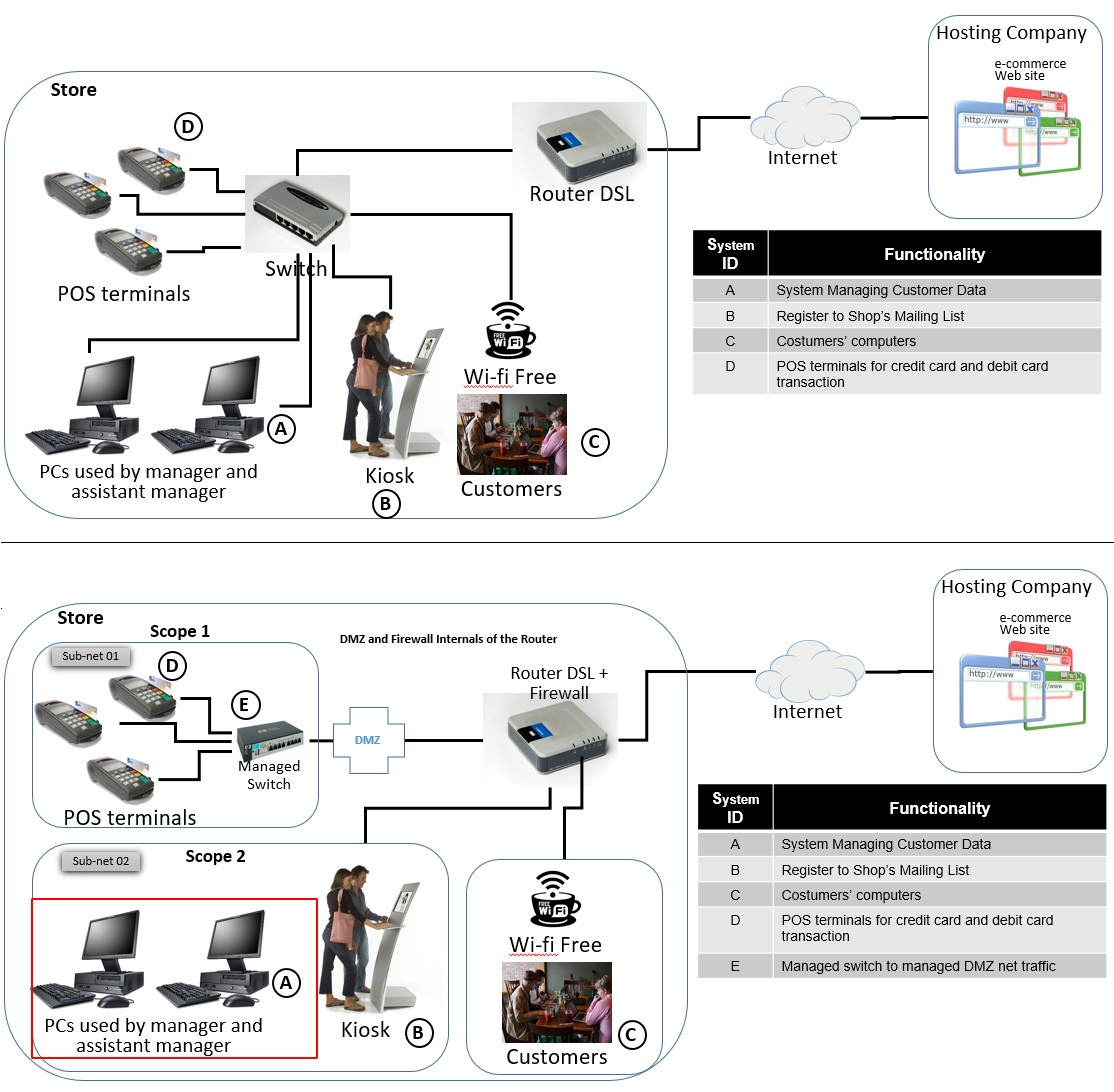
\includegraphics[width=0.92\linewidth]{figures/joebeforeandafter.jpg}
    \caption{Architecture of the Level 3 merchant network (Joe's Jumping Jerky Joint) before and after PCI-DSS network segmentation and DMZ enforcement~\cite{santos2017estimating, williams2014pci}.}
    \label{fig:app_joe_topology}
\end{figure}

\subsection{Architectural Remediation (After Compliance)}
To satisfy PCI-DSS scoping requirements (specifically Requirement 1 regarding firewall configurations and network segmentation), the merchant redeployed the infrastructure as shown in Figure~\ref{fig:app_joe_topology}:
\begin{enumerate}
    \item \textbf{Isolated POS DMZ Subnet:} The DMZ feature on the edge DSL router is activated. The IP-based POS devices are migrated to a dedicated, isolated physical subnet managed by an independent 8-port managed Ethernet switch.
    \item \textbf{Access Control and Ingress Filtering:} The DSL gateway firewall rules are locked down: no traffic originated from the administrative workstations, the kiosk, or the customer Wi-Fi is permitted to reach the POS devices or the POS controller.
    \item \textbf{Complete Wireless Isolation:} Guest Wi-Fi access is isolated into an independent logical broadcast domain with direct egress to the Internet, eliminating any local route to store management systems.
\end{enumerate}

\section{Scenario 2: Christine's Enterprise (Merchant Level 1)}
\label{sec:app_christine_scenario}
\subsection{Organizational Context and Core Switching Architecture}
Christine's company is a nationwide retail enterprise that expanded into a Merchant Level 1 organization. An internal security audit revealed that assessors had systematically underestimated the scope of PCI-DSS compliance because the corporate network was historically operated as a flat, unsegmented switching fabric.

Multiple legacy systems not involved in payment processing resided on the core corporate network. Because these legacy systems were no longer maintained by vendor software patches, they could not satisfy baseline PCI requirements. 

\begin{figure}[htbp]
    \centering
    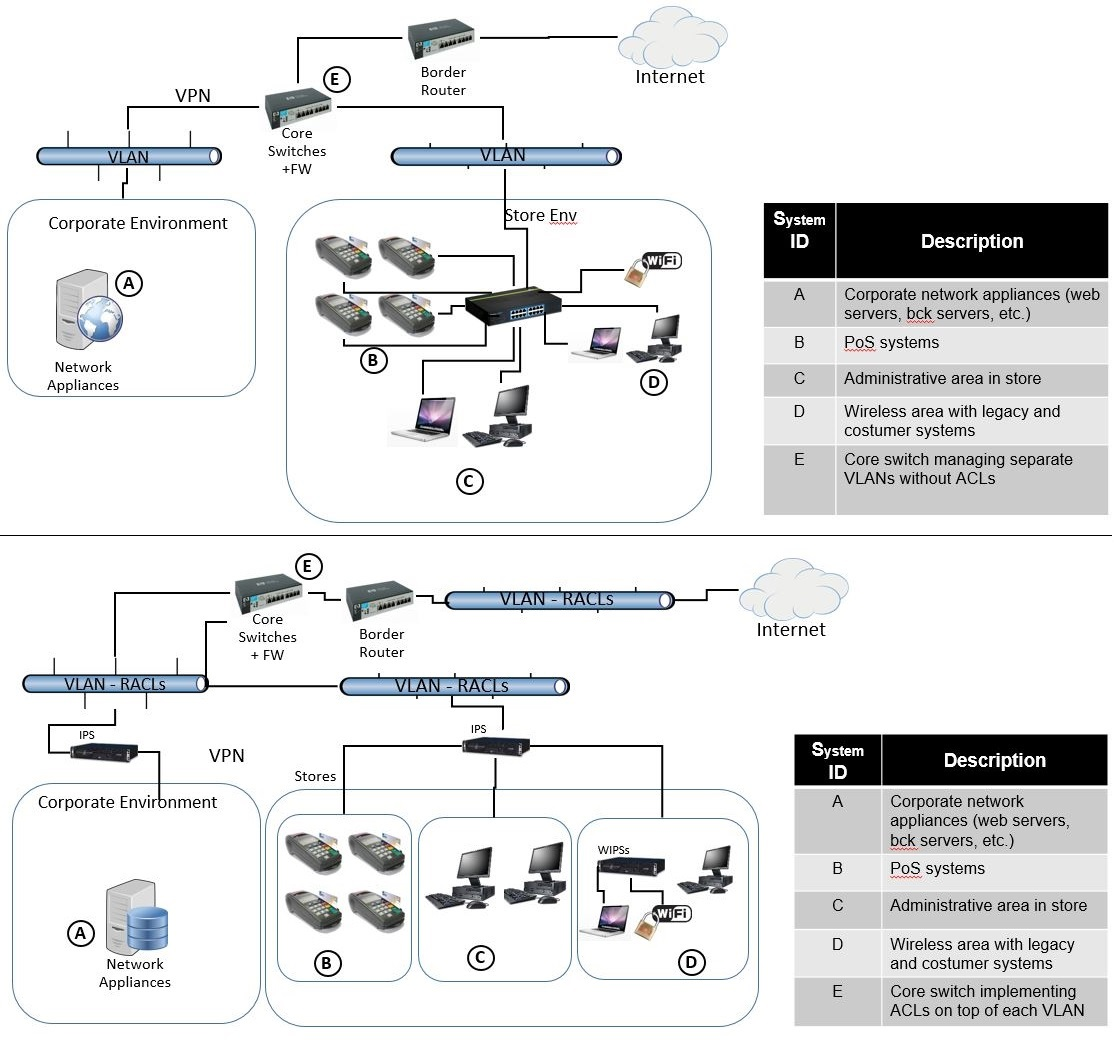
\includegraphics[width=0.95\linewidth]{figures/christinebeforeandafter.jpg}
    \caption{Architecture of the multi-tier enterprise network (Christine's Company) before and after core multi-VLAN segmentation and Router Access Control Lists (RACLs)~\cite{santos2017estimating, williams2014pci}.}
    \label{fig:app_christine_topology}
\end{figure}

\subsection{Multi-VLAN Remediation and RACL Enforcement}
To achieve compliance without undertaking a multi-million-dollar replacement of non-payment legacy systems, the enterprise deployed high-density aggregation switches (Cisco ASR series) equipped with hardware-enforced Router Access Control Lists (RACLs) and stateful firewall blades (Figure~\ref{fig:app_christine_topology}):
\begin{enumerate}
    \item \textbf{Cardholder Enclave Isolation:} The central payment processing servers and cardholder data repositories are isolated into dedicated VLANs protected by stateful inspection.
    \item \textbf{In-Store Point-of-Sale Segmentation:} Retail stores enforce RACLs that physically segregate POS terminals from administrative PCs and store kiosks.
    \item \textbf{Wireless Intrusion Prevention (WIPS):} Rogue access point detection and strict RACLs are activated across wireless access points to prevent air-interface bridging into the wired cardholder network.
    \item \textbf{Two-Factor VPN Bastion for Operators:} Technical administrators requiring access to cardholder systems are restricted to an Out-of-Band (OOB) management VRF protected by mandatory multi-factor authentication tokens.
\end{enumerate}

\chapter{Statistical Methodology and Replication Analysis}
\label{app:statistical_methods}

This appendix presents the complete mathematical formulations, hypotheses tests, and computational replication procedures underpinning both the historical human evaluator benchmark by Allodi et al.~\cite{santos2017estimating} and the HelpUS validation engine.

\section{Hypothesis Formulation and Fisher's Exact Test}
\label{sec:fisher_formulation}
To test whether human evaluators systematically fail when assessing vulnerabilities in complex environments, the evaluation is formalized as a series of $2 \times 2$ contingency tables. Let the assessment outcome for any participant evaluating vulnerability $v$ in network context $cxty \in \{\text{Flat}, \text{Segmented}\}$ be a binary random variable $Y \in \{0, 1\}$, where $Y = 1$ denotes agreement with the verified expert standard (correct) and $Y = 0$ denotes disagreement (incorrect).

\subsection{Network Complexity Hypothesis ($H2$)}
The null hypothesis states that the probability of correct assessment is independent of network topology:
\begin{align}
    H2_0: \quad & P(Y = 1 \mid \text{Flat}) = P(Y = 1 \mid \text{Segmented}) \\
    H2_1: \quad & P(Y = 1 \mid \text{Flat}) \neq P(Y = 1 \mid \text{Segmented})
\end{align}

Table~\ref{tab:app_contingency_network} summarizes the empirical contingency counts observed across the $n=29$ evaluator cohort ($N=348$ total scored instances).

\begin{table}[htbp]
\centering
\caption{Contingency Table of Assessment Correctness by Network Complexity}
\label{tab:app_contingency_network}
\begin{tabular}{lccc}
\toprule
\textbf{Network Architecture} & \textbf{Correct ($Y=1$)} & \textbf{Incorrect ($Y=0$)} & \textbf{Total} \\
\midrule
Flat (Simple)         & $a = 96$  & $b = 20$  & $n_1 = 116$ \\
Segmented (Complex)   & $c = 136$ & $d = 96$  & $n_2 = 232$ \\
\midrule
\textbf{Total}        & $m_1 = 232$ & $m_2 = 116$ & $N = 348$ \\
\bottomrule
\end{tabular}
\end{table}

Fisher's exact test computes the hypergeometric probability of observing the table marginals under $H2_0$:
\begin{equation}
    p = \frac{\binom{a+b}{a} \binom{c+d}{c}}{\binom{N}{a+c}} = \frac{\binom{116}{96} \binom{232}{136}}{\binom{348}{232}}
\end{equation}
The reproducibility script bundled with the project computes the two-sided Fisher exact test and both sample and conditional odds-ratio quantities. The generated values are:
\begin{align}
    p_{\text{Fisher, two-sided}} &= \HistFisherPScientific, \\n    \text{OR}_{\text{sample}} &= \HistSampleOR, \\n    \text{OR}_{\text{conditional MLE}} &= \HistConditionalOR.
\end{align}
Using the conditional exact method implemented by the pinned statistical toolchain, the $95\%$ confidence interval is:
\begin{equation}
    \text{CI}_{95\%,\text{conditional exact}} = [\HistConditionalCILow, \HistConditionalCIHigh].
\end{equation}
The method label is reported explicitly because this interval is not the same object as the simple asymptotic Wald interval. The historical null hypothesis of independence is rejected for this contingency table.

\section{Permutation Two-Way ANOVA for Co-Factor Invariance}
\label{sec:permutation_anova}
To ensure that the human error rate was not driven by individual demographic confounding factors (e.g., years of prior industry experience or self-reported security proficiency), the evaluation executed a non-parametric \textbf{Permutation Two-Way ANOVA}.

Let $F_{\text{obs}}$ denote the observed test statistic for the interaction between network scenario complexity and participant security experience. The null distribution is generated by randomly permuting the participant labels across $B = 10,000$ resamples:
\begin{equation}
    p_{\text{perm}} = \frac{1}{B} \sum_{b=1}^{B} \mathbb{I}\left( F^{(b)} \ge F_{\text{obs}} \right)
\end{equation}
The original participant-level data and complete permutation outputs are required to reproduce this co-factor analysis. Until those artifacts are included, this result should be treated as a historical-study claim rather than a newly reproduced HelpUS result.

\section{Monte Carlo Dispersal Simulation Algorithm}
\label{sec:monte_carlo_algo}
The synthetic score-space dispersal is generated by Algorithm~\ref{alg:monte_carlo}. It is a sensitivity simulation and is not the empirical distribution of human participant scores.

\begin{algorithm}[H]
\caption{Monte Carlo Scoring Dispersal Simulation}
\label{alg:monte_carlo}
\begin{algorithmic}[1]
\Require Base Score $S_{\text{base}}$, Permutation Count $N = 10,000$, Topology Type $\mathcal{T}$
\Ensure Score Distribution Vector $\mathbf{S}_{\text{dist}}$
\State $\mathbf{S}_{\text{dist}} \gets \emptyset$
\For{$i = 1$ to $N$}
    \State Sample $\text{CR} \sim \mathcal{U}\{\text{High}, \text{Medium}, \text{Low}\}$
    \State Sample $\text{IR} \sim \mathcal{U}\{\text{High}, \text{Medium}, \text{Low}\}$
    \State Sample $\text{AR} \sim \mathcal{U}\{\text{High}, \text{Medium}, \text{Low}\}$
    \If{$\mathcal{T} = \text{Segmented}$}
        \State Sample $\text{MAV} \sim \mathcal{U}\{\text{Network}, \text{Adjacent}, \text{Local}\}$
    \Else
        \State $\text{MAV} \gets \text{Network}$
    \EndIf
    \State $S_{\text{sim}} \gets \text{ComputeCVSS40}(S_{\text{base}}, \text{MAV}, \text{CR}, \text{IR}, \text{AR})$
    \State $\mathbf{S}_{\text{dist}} \gets \mathbf{S}_{\text{dist}} \cup \{S_{\text{sim}}\}$
\EndFor
\State \Return $\mathbf{S}_{\text{dist}}$
\end{algorithmic}
\end{algorithm}

\chapter{Complete Experimental Datasets}
\label{app:historical_dataset}

This appendix summarizes the current benchmark corpus. Full computational reproducibility additionally requires machine-readable source vectors, source/retrieval metadata, evidence objects, rule versions, calculator version, scripts, and independent reference labels. Those artifacts should accompany the final paper release.

\section{Historical 2017 Vulnerability Corpus (Allodi et al.)}
\label{sec:app_historical_cves}
Table~\ref{tab:app_historical_cves} documents the complete set of twelve Common Vulnerabilities and Exposures (CVEs) evaluated during the controlled trials across flat and segmented topologies~\cite{santos2017estimating}.

\begin{landscape}
\begin{table}[p]
\centering\scriptsize
\caption{Historical Vulnerability Dataset from the Allodi et al.~\cite{santos2017estimating} Empirical Trial}
\label{tab:app_historical_cves}
\begin{adjustbox}{max width=\linewidth}
\begin{tabular}{lp{3.5cm}p{2.8cm}ccp{3.7cm}p{2.6cm}}
\toprule
\textbf{CVE ID} & \textbf{Affected Software} & \textbf{Target Host} & \textbf{Type} & \textbf{Base} & \textbf{CVSS Vector} & \textbf{Observed Human Error} \\
\midrule
CVE-2016-0126 & Microsoft Office 2016 & Customer Data PC & APP & 7.8 & AV:L/\allowbreak AC:L/\allowbreak PR:N/\allowbreak UI:R & 10.0\% \\
CVE-2016-5167 & Google Chrome 53      & Mailing Kiosk    & APP & 8.8 & AV:N/\allowbreak AC:L/\allowbreak PR:N/\allowbreak UI:R & 21.0\% \\
CVE-2016-0019 & Windows 10 Workstation& Customer PC      & SYS & 8.1 & AV:N/\allowbreak AC:H/\allowbreak PR:N/\allowbreak UI:N & 28.0\% \\
CVE-2016-0067 & POS Terminal System   & Store POS IP     & SYS & 7.8 & AV:L/\allowbreak AC:L/\allowbreak PR:L/\allowbreak UI:N & 10.0\% \\
CVE-2016-0036 & Windows Server 2012   & Corporate Server & SYS & 8.8 & AV:N/\allowbreak AC:L/\allowbreak PR:L/\allowbreak UI:N & 76.0\% \\
CVE-2016-0469 & Oracle Retail MICROS  & Retail Store POS & SYS & 5.5 & AV:L/\allowbreak AC:L/\allowbreak PR:L/\allowbreak UI:N & 79.0\% \\
CVE-2016-3234 & Microsoft Office 2010 & Store Admin PC   & APP & 5.5 & AV:L/\allowbreak AC:L/\allowbreak PR:N/\allowbreak UI:R & 45.0\% \\
CVE-2016-6792 & Google Chrome 47      & Store Admin PC   & APP & 9.8 & AV:N/\allowbreak AC:L/\allowbreak PR:N/\allowbreak UI:N & 86.0\% \\
CVE-2016-0012 & Microsoft Office 2010 & Legacy Wi-Fi PC  & APP & 4.3 & AV:N/\allowbreak AC:L/\allowbreak PR:N/\allowbreak UI:R & 34.0\% \\
CVE-2016-1619 & Google Chrome 48      & Legacy Wi-Fi PC  & APP & 7.6 & AV:N/\allowbreak AC:L/\allowbreak PR:N/\allowbreak UI:R & 83.0\% \\
CVE-2016-6441 & Cisco IOS XE (ASR 900)& Core VLAN Switch & SYS & 9.8 & AV:N/\allowbreak AC:L/\allowbreak PR:N/\allowbreak UI:N & 86.0\% \\
CVE-2016-6428 & Cisco IOS XR          & Core VLAN Switch & SYS & 7.8 & AV:L/\allowbreak AC:L/\allowbreak PR:L/\allowbreak UI:N & 90.0\% \\
\bottomrule
\end{tabular}
\end{adjustbox}
\end{table}
\end{landscape}

\section{Dataset B: 30-Scenario Development Benchmark}
\label{sec:app_modern_benchmark}
Dataset B is a development/regression benchmark rather than a held-out validation set. Its canonical schema separates provider-reported Base values from scores recomputed from the full source vector. This distinction is essential for CVSS-BT records: a provider may publish a Base score while the complete source vector also defines Threat metric $E$, yielding a different Base+Threat score. The synthetic fixtures also preserve their legacy investigator-assigned scores separately from the current vector recomputation. Several of those legacy assigned scores do not match the score recomputed from their own vectors; the discrepancy is intentionally exposed rather than silently overwritten and must be normalized only after calculator gate G1 closes with the final pinned scorer. The tables below are generated from the schema-v2 machine-readable dataset bundled with this monograph.

\begin{landscape}
\begin{table}[p]
\centering\scriptsize
\caption{Dataset B real-CVE source-assessment provenance (12 development scenarios). Provider-reported Base values are kept distinct from scores recomputed from the complete source vector. Full-vector recomputation remains provisional until calculator gate G1 reaches zero unexplained FIRST-reference mismatches.}
\label{tab:dataset_b_v2_real}
\begin{adjustbox}{max width=\linewidth}
\begin{tabular}{llllllll}
\toprule
\textbf{Scenario} & \textbf{CVE} & \textbf{Provider} & \textbf{Nom.} & \textbf{Provider Base} & \textbf{Current Full Vector} & \textbf{Full Sev.} & \textbf{Disposition} \\
\midrule
SCN-NVD-001 & CVE-2026-4251 & cna@vuldb.com & CVSS-BT & 2.0 & 1.1 & Low & P3 \\
SCN-NVD-002 & CVE-2026-4252 & cna@vuldb.com & CVSS-BT & 9.3 & 8.9 & High & P2 \\
SCN-NVD-003 & CVE-2026-4270 & ff89ba41-3aa1-4d27-914a-91399e9639e5 & CVSS-B & 6.8 & 6.8 & Medium & P1 \\
SCN-NVD-004 & CVE-2026-28490 & security-advisories@github.com & CVSS-B & 8.3 & 8.3 & High & P0 \\
SCN-NVD-005 & CVE-2026-28498 & security-advisories@github.com & CVSS-B & 8.2 & 8.2 & High & P1 \\
SCN-NVD-006 & CVE-2026-29510 & disclosure@vulncheck.com & CVSS-B & 5.1 & 5.1 & Medium & P3 \\
SCN-NVD-007 & CVE-2026-29513 & disclosure@vulncheck.com & CVSS-B & 5.1 & 5.1 & Medium & P2 \\
SCN-NVD-008 & CVE-2026-29520 & disclosure@vulncheck.com & CVSS-B & 5.1 & 5.1 & Medium & P1 \\
SCN-NVD-009 & CVE-2026-29521 & disclosure@vulncheck.com & CVSS-B & 5.1 & 5.1 & Medium & P1 \\
SCN-NVD-010 & CVE-2026-3644 & cna@python.org & CVSS-B & 6.0 & 6.0 & Medium & P3 \\
SCN-NVD-011 & CVE-2026-4224 & cna@python.org & CVSS-B & 6.0 & 6.0 & Medium & P1 \\
SCN-NVD-012 & CVE-2026-4253 & cna@vuldb.com & CVSS-BT & 5.1 & 2.0 & Low & P2 \\
\bottomrule
\end{tabular}
\end{adjustbox}
\end{table}
\end{landscape}

\begin{landscape}
\begin{table}[p]
\centering\scriptsize
\caption{Dataset B synthetic development scenarios (18 fixtures). The legacy assigned score is retained for provenance; the current vector recomputation exposes inconsistencies that must be resolved after calculator gate G1 closes. Synthetic inputs are investigator-authored and are not CNA/NVD-published assessments.}
\label{tab:dataset_b_v2_synth}
\begin{adjustbox}{max width=\linewidth}
\begin{tabular}{llllllll}
\toprule
\textbf{Scenario} & \textbf{Asset Class} & \textbf{Nom.} & \textbf{Legacy Assigned} & \textbf{Current Recompute} & \textbf{Legacy Sev.} & \textbf{Current Sev.} & \textbf{Disposition} \\
\midrule
SCN-SYN-013 & developer\_workstation & CVSS-B & 9.3 & 10.0 & Critical & Critical & P0 \\
SCN-SYN-014 & isolated\_lab\_system & CVSS-B & 8.7 & 9.4 & High & Critical & P4 \\
SCN-SYN-015 & ot\_monitoring\_gateway & CVSS-B & 7.1 & 8.4 & High & High & P0 \\
SCN-SYN-016 & public\_api\_gateway & CVSS-B & 6.8 & 8.4 & Medium & High & P0 \\
SCN-SYN-017 & public\_web\_application & CVSS-B & 4.8 & 2.0 & Medium & Low & P1 \\
SCN-SYN-018 & internal\_admin\_console & CVSS-B & 2.1 & 1.0 & Low & Low & P4 \\
SCN-SYN-019 & identity\_provider & CVSS-B & 9.3 & 10.0 & Critical & Critical & P0 \\
SCN-SYN-020 & database\_server & CVSS-B & 8.7 & 9.4 & High & Critical & P0 \\
SCN-SYN-021 & developer\_workstation & CVSS-B & 7.1 & 8.4 & High & High & P1 \\
SCN-SYN-022 & isolated\_lab\_system & CVSS-B & 6.8 & 8.4 & Medium & High & P4 \\
SCN-SYN-023 & ot\_monitoring\_gateway & CVSS-B & 4.8 & 2.0 & Medium & Low & P0 \\
SCN-SYN-024 & public\_api\_gateway & CVSS-B & 2.1 & 1.0 & Low & Low & P1 \\
SCN-SYN-025 & public\_web\_application & CVSS-B & 9.3 & 10.0 & Critical & Critical & P0 \\
SCN-SYN-026 & internal\_admin\_console & CVSS-B & 8.7 & 9.4 & High & Critical & P2 \\
SCN-SYN-027 & identity\_provider & CVSS-B & 7.1 & 8.4 & High & High & P0 \\
SCN-SYN-028 & database\_server & CVSS-B & 6.8 & 8.4 & Medium & High & P1 \\
SCN-SYN-029 & developer\_workstation & CVSS-B & 4.8 & 2.0 & Medium & Low & P2 \\
SCN-SYN-030 & isolated\_lab\_system & CVSS-B & 2.1 & 1.0 & Low & Low & P4 \\
\bottomrule
\end{tabular}
\end{adjustbox}
\end{table}
\end{landscape}



\backmatter

\bibliographystyle{IEEEtran}
\bibliography{references}

\end{document}
